\documentclass[1p]{elsarticle_modified}
%\bibliographystyle{elsarticle-num}

%\usepackage[colorlinks]{hyperref}
%\usepackage{abbrmath_seonhwa} %\Abb, \Ascr, \Acal ,\Abf, \Afrak
\usepackage{amsfonts}
\usepackage{amssymb}
\usepackage{amsmath}
\usepackage{amsthm}
\usepackage{scalefnt}
\usepackage{amsbsy}
\usepackage{kotex}
\usepackage{caption}
\usepackage{subfig}
\usepackage{color}
\usepackage{graphicx}
\usepackage{xcolor} %% white, black, red, green, blue, cyan, magenta, yellow
\usepackage{float}
\usepackage{setspace}
\usepackage{hyperref}

\usepackage{tikz}
\usetikzlibrary{arrows}

\usepackage{multirow}
\usepackage{array} % fixed length table
\usepackage{hhline}

%%%%%%%%%%%%%%%%%%%%%
\makeatletter
\renewcommand*\env@matrix[1][\arraystretch]{%
	\edef\arraystretch{#1}%
	\hskip -\arraycolsep
	\let\@ifnextchar\new@ifnextchar
	\array{*\c@MaxMatrixCols c}}
\makeatother %https://tex.stackexchange.com/questions/14071/how-can-i-increase-the-line-spacing-in-a-matrix
%%%%%%%%%%%%%%%

\usepackage[normalem]{ulem}

\newcommand{\msout}[1]{\ifmmode\text{\sout{\ensuremath{#1}}}\else\sout{#1}\fi}
%SOURCE: \msout is \stkout macro in https://tex.stackexchange.com/questions/20609/strikeout-in-math-mode

\newcommand{\cancel}[1]{
	\ifmmode
	{\color{red}\msout{#1}}
	\else
	{\color{red}\sout{#1}}
	\fi
}

\newcommand{\add}[1]{
	{\color{blue}\uwave{#1}}
}

\newcommand{\replace}[2]{
	\ifmmode
	{\color{red}\msout{#1}}{\color{blue}\uwave{#2}}
	\else
	{\color{red}\sout{#1}}{\color{blue}\uwave{#2}}
	\fi
}

\newcommand{\Sol}{\mathcal{S}} %segment
\newcommand{\D}{D} %diagram
\newcommand{\A}{\mathcal{A}} %arc


%%%%%%%%%%%%%%%%%%%%%%%%%%%%%5 test

\def\sl{\operatorname{\textup{SL}}(2,\Cbb)}
\def\psl{\operatorname{\textup{PSL}}(2,\Cbb)}
\def\quan{\mkern 1mu \triangleright \mkern 1mu}

\theoremstyle{definition}
\newtheorem{thm}{Theorem}[section]
\newtheorem{prop}[thm]{Proposition}
\newtheorem{lem}[thm]{Lemma}
\newtheorem{ques}[thm]{Question}
\newtheorem{cor}[thm]{Corollary}
\newtheorem{defn}[thm]{Definition}
\newtheorem{exam}[thm]{Example}
\newtheorem{rmk}[thm]{Remark}
\newtheorem{alg}[thm]{Algorithm}

\newcommand{\I}{\sqrt{-1}}
\begin{document}

%\begin{frontmatter}
%
%\title{Boundary parabolic representations of knots up to 8 crossings}
%
%%% Group authors per affiliation:
%\author{Yunhi Cho} 
%\address{Department of Mathematics, University of Seoul, Seoul, Korea}
%\ead{yhcho@uos.ac.kr}
%
%
%\author{Seonhwa Kim} %\fnref{s_kim}}
%\address{Center for Geometry and Physics, Institute for Basic Science, Pohang, 37673, Korea}
%\ead{ryeona17@ibs.re.kr}
%
%\author{Hyuk Kim}
%\address{Department of Mathematical Sciences, Seoul National University, Seoul 08826, Korea}
%\ead{hyukkim@snu.ac.kr}
%
%\author{Seokbeom Yoon}
%\address{Department of Mathematical Sciences, Seoul National University, Seoul, 08826,  Korea}
%\ead{sbyoon15@snu.ac.kr}
%
%\begin{abstract}
%We find all boundary parabolic representation of knots up to 8 crossings.
%
%\end{abstract}
%\begin{keyword}
%    \MSC[2010] 57M25 
%\end{keyword}
%
%\end{frontmatter}

%\linenumbers
%\tableofcontents
%
\newcommand\colored[1]{\textcolor{white}{\rule[-0.35ex]{0.8em}{1.4ex}}\kern-0.8em\color{red} #1}%
%\newcommand\colored[1]{\textcolor{white}{ #1}\kern-2.17ex	\textcolor{white}{ #1}\kern-1.81ex	\textcolor{white}{ #1}\kern-2.15ex\color{red}#1	}

{\Large $\underline{12a_{1180}~(K12a_{1180})}$}

\setlength{\tabcolsep}{10pt}
\renewcommand{\arraystretch}{1.6}
\vspace{1cm}\begin{tabular}{m{100pt}>{\centering\arraybackslash}m{274pt}}
\multirow{5}{120pt}{
	\centering
	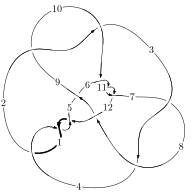
\includegraphics[width=112pt]{../../../GIT/diagram.site/Diagrams/png/1981_12a_1180.png}\\
\ \ \ A knot diagram\footnotemark}&
\allowdisplaybreaks
\textbf{Linearized knot diagam} \\
\cline{2-2}
 &
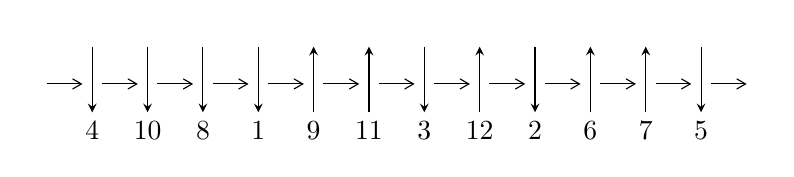
\begin{tikzpicture}[x=20pt, y=17pt]
	% nodes
	\node (C0) at (0, 0) {};
	\node (C1) at (1, 0) {};
	\node (C1U) at (1, +1) {};
	\node (C1D) at (1, -1) {4};

	\node (C2) at (2, 0) {};
	\node (C2U) at (2, +1) {};
	\node (C2D) at (2, -1) {10};

	\node (C3) at (3, 0) {};
	\node (C3U) at (3, +1) {};
	\node (C3D) at (3, -1) {8};

	\node (C4) at (4, 0) {};
	\node (C4U) at (4, +1) {};
	\node (C4D) at (4, -1) {1};

	\node (C5) at (5, 0) {};
	\node (C5U) at (5, +1) {};
	\node (C5D) at (5, -1) {9};

	\node (C6) at (6, 0) {};
	\node (C6U) at (6, +1) {};
	\node (C6D) at (6, -1) {11};

	\node (C7) at (7, 0) {};
	\node (C7U) at (7, +1) {};
	\node (C7D) at (7, -1) {3};

	\node (C8) at (8, 0) {};
	\node (C8U) at (8, +1) {};
	\node (C8D) at (8, -1) {12};

	\node (C9) at (9, 0) {};
	\node (C9U) at (9, +1) {};
	\node (C9D) at (9, -1) {2};

	\node (C10) at (10, 0) {};
	\node (C10U) at (10, +1) {};
	\node (C10D) at (10, -1) {6};

	\node (C11) at (11, 0) {};
	\node (C11U) at (11, +1) {};
	\node (C11D) at (11, -1) {7};

	\node (C12) at (12, 0) {};
	\node (C12U) at (12, +1) {};
	\node (C12D) at (12, -1) {5};
	\node (C13) at (13, 0) {};

	% arrows
	\draw[->,>={angle 60}]
	(C0) edge (C1) (C1) edge (C2) (C2) edge (C3) (C3) edge (C4) (C4) edge (C5) (C5) edge (C6) (C6) edge (C7) (C7) edge (C8) (C8) edge (C9) (C9) edge (C10) (C10) edge (C11) (C11) edge (C12) (C12) edge (C13) ;	\draw[->,>=stealth]
	(C1U) edge (C1D) (C2U) edge (C2D) (C3U) edge (C3D) (C4U) edge (C4D) (C5D) edge (C5U) (C6D) edge (C6U) (C7U) edge (C7D) (C8D) edge (C8U) (C9U) edge (C9D) (C10D) edge (C10U) (C11D) edge (C11U) (C12U) edge (C12D) ;
	\end{tikzpicture} \\
\hhline{~~} \\& 
\textbf{Solving Sequence} \\ \cline{2-2} 
 &
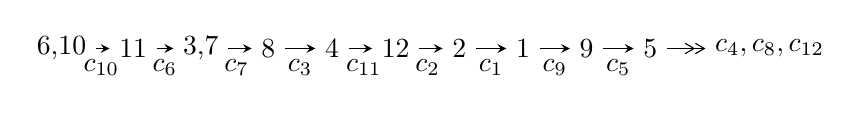
\begin{tikzpicture}[x=23pt, y=7pt]
	% node
	\node (A0) at (-1/8, 0) {6,10};
	\node (A1) at (1, 0) {11};
	\node (A2) at (33/16, 0) {3,7};
	\node (A3) at (25/8, 0) {8};
	\node (A4) at (33/8, 0) {4};
	\node (A5) at (41/8, 0) {12};
	\node (A6) at (49/8, 0) {2};
	\node (A7) at (57/8, 0) {1};
	\node (A8) at (65/8, 0) {9};
	\node (A9) at (73/8, 0) {5};
	\node (C1) at (1/2, -1) {$c_{10}$};
	\node (C2) at (3/2, -1) {$c_{6}$};
	\node (C3) at (21/8, -1) {$c_{7}$};
	\node (C4) at (29/8, -1) {$c_{3}$};
	\node (C5) at (37/8, -1) {$c_{11}$};
	\node (C6) at (45/8, -1) {$c_{2}$};
	\node (C7) at (53/8, -1) {$c_{1}$};
	\node (C8) at (61/8, -1) {$c_{9}$};
	\node (C9) at (69/8, -1) {$c_{5}$};
	\node (A10) at (11, 0) {$c_{4},c_{8},c_{12}$};

	% edge
	\draw[->,>=stealth]	
	(A0) edge (A1) (A1) edge (A2) (A2) edge (A3) (A3) edge (A4) (A4) edge (A5) (A5) edge (A6) (A6) edge (A7) (A7) edge (A8) (A8) edge (A9) ;
	\draw[->>,>={angle 60}]	
	(A9) edge (A10);
\end{tikzpicture} \\ 

\end{tabular} \\

\footnotetext{
The image of knot diagram is generated by the software ``\textbf{Draw programme}" developed by Andrew Bartholomew(\url{http://www.layer8.co.uk/maths/draw/index.htm\#Running-draw}), where we modified some parts for our purpose(\url{https://github.com/CATsTAILs/LinksPainter}).
}\phantom \\ \newline 
\centering \textbf{Ideals for irreducible components\footnotemark of $X_{\text{par}}$} 
 
\begin{align*}
I^u_{1}&=\langle 
40129 u^{36}+541351 u^{35}+\cdots+64 b+3448384,\\
\phantom{I^u_{1}}&\phantom{= \langle  }-117149 u^{36}-1586205 u^{35}+\cdots+128 a-10309184,\;u^{37}+15 u^{36}+\cdots+128 u+128\rangle \\
I^u_{2}&=\langle 
-2589926063 a^5 u^4+1727557591 a^4 u^4+\cdots+14756925898 a+2746218374,\\
\phantom{I^u_{2}}&\phantom{= \langle  }a^4 u^4+2 u^4 a^3+\cdots-2 a+5,\;u^5- u^4-2 u^3+u^2+u+1\rangle \\
I^u_{3}&=\langle 
-1.25456\times10^{19} a^{7} u^{4}-3.69023\times10^{18} a^{6} u^{4}+\cdots-3.06241\times10^{19} a+1.52681\times10^{20},\\
\phantom{I^u_{3}}&\phantom{= \langle  }a^7 u^4+3 a^6 u^4+\cdots+5 a-2,\;u^5- u^4-2 u^3+u^2+u+1\rangle \\
I^u_{4}&=\langle 
-3 u^{24}+5 u^{23}+\cdots+b-3,\;-3 u^{23}+37 u^{21}+\cdots+a+1,\;u^{25}-14 u^{23}+\cdots-6 u^2+1\rangle \\
\\
\end{align*}
\raggedright * 4 irreducible components of $\dim_{\mathbb{C}}=0$, with total 132 representations.\\
\footnotetext{All coefficients of polynomials are rational numbers. But the coefficients are sometimes approximated in decimal forms when there is not enough margin.}
\newpage
\renewcommand{\arraystretch}{1}
\centering \section*{I. $I^u_{1}= \langle 40129 u^{36}+541351 u^{35}+\cdots+64 b+3448384,\;-1.17\times10^{5} u^{36}-1.59\times10^{6} u^{35}+\cdots+128 a-1.03\times10^{7},\;u^{37}+15 u^{36}+\cdots+128 u+128 \rangle$}
\flushleft \textbf{(i) Arc colorings}\\
\begin{tabular}{m{7pt} m{180pt} m{7pt} m{180pt} }
\flushright $a_{6}=$&$\begin{pmatrix}0\\u\end{pmatrix}$ \\
\flushright $a_{10}=$&$\begin{pmatrix}1\\0\end{pmatrix}$ \\
\flushright $a_{11}=$&$\begin{pmatrix}1\\- u^2\end{pmatrix}$ \\
\flushright $a_{3}=$&$\begin{pmatrix}915.227 u^{36}+12392.2 u^{35}+\cdots+25110.5 u+80540.5\\-627.016 u^{36}-8458.61 u^{35}+\cdots-17272.5 u-53881\end{pmatrix}$ \\
\flushright $a_{7}=$&$\begin{pmatrix}u\\- u^3+u\end{pmatrix}$ \\
\flushright $a_{8}=$&$\begin{pmatrix}-8.50000 u^{36}-98.5000 u^{35}+\cdots-495.500 u+160.500\\\frac{157}{4} u^{36}+518 u^{35}+\cdots+\frac{2753}{2} u+2624\end{pmatrix}$ \\
\flushright $a_{4}=$&$\begin{pmatrix}503.828 u^{36}+6655.03 u^{35}+\cdots+16741.3 u+34828\\-165.578 u^{36}-2187.45 u^{35}+\cdots-6821 u-10106\end{pmatrix}$ \\
\flushright $a_{12}=$&$\begin{pmatrix}- u^2+1\\u^4-2 u^2\end{pmatrix}$ \\
\flushright $a_{2}=$&$\begin{pmatrix}288.211 u^{36}+3933.62 u^{35}+\cdots+7838 u+26659.5\\-627.016 u^{36}-8458.61 u^{35}+\cdots-17272.5 u-53881\end{pmatrix}$ \\
\flushright $a_{1}=$&$\begin{pmatrix}-410.313 u^{36}-5606.69 u^{35}+\cdots-11464 u-37783\\-\frac{3733}{16} u^{36}-\frac{24335}{8} u^{35}+\cdots-8416 u-13816\end{pmatrix}$ \\
\flushright $a_{9}=$&$\begin{pmatrix}-\frac{123}{4} u^{36}-\frac{839}{2} u^{35}+\cdots-879 u-\frac{5567}{2}\\-\frac{157}{4} u^{36}-518 u^{35}+\cdots-\frac{2751}{2} u-2624\end{pmatrix}$ \\
\flushright $a_{5}=$&$\begin{pmatrix}\frac{285}{2} u^{36}+\frac{7613}{4} u^{35}+\cdots+\frac{18879}{4} u+10688\\-\frac{285}{4} u^{36}-\frac{2053}{2} u^{35}+\cdots-1055 u-9568\end{pmatrix}$\\&\end{tabular}
\flushleft \textbf{(ii) Obstruction class $= -1$}\\~\\
\flushleft \textbf{(iii) Cusp Shapes $= \frac{19693}{16} u^{36}+\frac{264633}{16} u^{35}+\cdots+34556 u+102558$}\\~\\
\newpage\renewcommand{\arraystretch}{1}
\flushleft \textbf{(iv) u-Polynomials at the component}\newline \\
\begin{tabular}{m{50pt}|m{274pt}}
Crossings & \hspace{64pt}u-Polynomials at each crossing \\
\hline $$\begin{aligned}c_{1},c_{4},c_{12}\end{aligned}$$&$\begin{aligned}
&u^{37}-12 u^{36}+\cdots+464 u-32
\end{aligned}$\\
\hline $$\begin{aligned}c_{2},c_{3},c_{7}\\c_{9}\end{aligned}$$&$\begin{aligned}
&u^{37}- u^{36}+\cdots+u-1
\end{aligned}$\\
\hline $$\begin{aligned}c_{5},c_{8}\end{aligned}$$&$\begin{aligned}
&u^{37}-15 u^{35}+\cdots+3 u+1
\end{aligned}$\\
\hline $$\begin{aligned}c_{6},c_{10},c_{11}\end{aligned}$$&$\begin{aligned}
&u^{37}+15 u^{36}+\cdots+128 u+128
\end{aligned}$\\
\hline
\end{tabular}\\~\\
\newpage\renewcommand{\arraystretch}{1}
\flushleft \textbf{(v) Riley Polynomials at the component}\newline \\
\begin{tabular}{m{50pt}|m{274pt}}
Crossings & \hspace{64pt}Riley Polynomials at each crossing \\
\hline $$\begin{aligned}c_{1},c_{4},c_{12}\end{aligned}$$&$\begin{aligned}
&y^{37}+32 y^{36}+\cdots-3328 y-1024
\end{aligned}$\\
\hline $$\begin{aligned}c_{2},c_{3},c_{7}\\c_{9}\end{aligned}$$&$\begin{aligned}
&y^{37}-19 y^{36}+\cdots+9 y-1
\end{aligned}$\\
\hline $$\begin{aligned}c_{5},c_{8}\end{aligned}$$&$\begin{aligned}
&y^{37}-30 y^{36}+\cdots+19 y-1
\end{aligned}$\\
\hline $$\begin{aligned}c_{6},c_{10},c_{11}\end{aligned}$$&$\begin{aligned}
&y^{37}-33 y^{36}+\cdots+65536 y-16384
\end{aligned}$\\
\hline
\end{tabular}\\~\\
\newpage\flushleft \textbf{(vi) Complex Volumes and Cusp Shapes}
$$\begin{array}{c|c|c}  
\text{Solutions to }I^u_{1}& \I (\text{vol} + \sqrt{-1}CS) & \text{Cusp shape}\\
 \hline 
\begin{aligned}
u &= \phantom{-}0.351636 + 0.943218 I \\
a &= -0.475955 - 0.640393 I \\
b &= -1.226050 + 0.499285 I\end{aligned}
 & -4.86867 + 8.36618 I & -5.40191 - 7.90416 I \\ \hline\begin{aligned}
u &= \phantom{-}0.351636 - 0.943218 I \\
a &= -0.475955 + 0.640393 I \\
b &= -1.226050 - 0.499285 I\end{aligned}
 & -4.86867 - 8.36618 I & -5.40191 + 7.90416 I \\ \hline\begin{aligned}
u &= \phantom{-}0.241715 + 0.981613 I \\
a &= \phantom{-}0.517408 + 0.493867 I \\
b &= \phantom{-}1.062410 - 0.425783 I\end{aligned}
 & -3.19836 + 3.03653 I & \phantom{-0.000000 } 0. - 4.95054 I \\ \hline\begin{aligned}
u &= \phantom{-}0.241715 - 0.981613 I \\
a &= \phantom{-}0.517408 - 0.493867 I \\
b &= \phantom{-}1.062410 + 0.425783 I\end{aligned}
 & -3.19836 - 3.03653 I & \phantom{-0.000000 -}0. + 4.95054 I \\ \hline\begin{aligned}
u &= \phantom{-}0.385505 + 0.899265 I \\
a &= \phantom{-}0.501965 + 0.739361 I \\
b &= \phantom{-}1.31533 - 0.59643 I\end{aligned}
 & \phantom{-}0.99167 + 12.76550 I & -2.00000 - 8.13132 I \\ \hline\begin{aligned}
u &= \phantom{-}0.385505 - 0.899265 I \\
a &= \phantom{-}0.501965 - 0.739361 I \\
b &= \phantom{-}1.31533 + 0.59643 I\end{aligned}
 & \phantom{-}0.99167 - 12.76550 I & -2.00000 + 8.13132 I \\ \hline\begin{aligned}
u &= \phantom{-}0.839963 + 0.746345 I \\
a &= \phantom{-}0.400856 - 0.379292 I \\
b &= -1.154870 - 0.426854 I\end{aligned}
 & \phantom{-}2.32825 - 7.20667 I & \phantom{-0.000000 } 0 \\ \hline\begin{aligned}
u &= \phantom{-}0.839963 - 0.746345 I \\
a &= \phantom{-}0.400856 + 0.379292 I \\
b &= -1.154870 + 0.426854 I\end{aligned}
 & \phantom{-}2.32825 + 7.20667 I & \phantom{-0.000000 } 0 \\ \hline\begin{aligned}
u &= -1.048710 + 0.504742 I \\
a &= -0.767420 + 0.920923 I \\
b &= -0.666422 - 0.237516 I\end{aligned}
 & \phantom{-}0.55587 - 4.70914 I & \phantom{-0.000000 } 0 \\ \hline\begin{aligned}
u &= -1.048710 - 0.504742 I \\
a &= -0.767420 - 0.920923 I \\
b &= -0.666422 + 0.237516 I\end{aligned}
 & \phantom{-}0.55587 + 4.70914 I & \phantom{-0.000000 } 0\\
 \hline 
 \end{array}$$\newpage$$\begin{array}{c|c|c}  
\text{Solutions to }I^u_{1}& \I (\text{vol} + \sqrt{-1}CS) & \text{Cusp shape}\\
 \hline 
\begin{aligned}
u &= \phantom{-}0.959859 + 0.749495 I \\
a &= -0.320732 + 0.294928 I \\
b &= \phantom{-}1.068580 + 0.312720 I\end{aligned}
 & -3.11272 - 2.58575 I & \phantom{-0.000000 } 0 \\ \hline\begin{aligned}
u &= \phantom{-}0.959859 - 0.749495 I \\
a &= -0.320732 - 0.294928 I \\
b &= \phantom{-}1.068580 - 0.312720 I\end{aligned}
 & -3.11272 + 2.58575 I & \phantom{-0.000000 } 0 \\ \hline\begin{aligned}
u &= \phantom{-}0.611888 + 0.466895 I \\
a &= -0.692399 - 0.072885 I \\
b &= \phantom{-}0.456299 + 0.774896 I\end{aligned}
 & \phantom{-}6.65717 + 1.91106 I & \phantom{-}4.08301 - 1.85461 I \\ \hline\begin{aligned}
u &= \phantom{-}0.611888 - 0.466895 I \\
a &= -0.692399 + 0.072885 I \\
b &= \phantom{-}0.456299 - 0.774896 I\end{aligned}
 & \phantom{-}6.65717 - 1.91106 I & \phantom{-}4.08301 + 1.85461 I \\ \hline\begin{aligned}
u &= \phantom{-}0.226538 + 0.683581 I \\
a &= -0.823439 - 0.518819 I \\
b &= -0.671321 + 0.719640 I\end{aligned}
 & \phantom{-}5.38858 + 1.85504 I & \phantom{-}1.65918 - 4.21077 I \\ \hline\begin{aligned}
u &= \phantom{-}0.226538 - 0.683581 I \\
a &= -0.823439 + 0.518819 I \\
b &= -0.671321 - 0.719640 I\end{aligned}
 & \phantom{-}5.38858 - 1.85504 I & \phantom{-}1.65918 + 4.21077 I \\ \hline\begin{aligned}
u &= \phantom{-}1.155400 + 0.665505 I \\
a &= \phantom{-}0.270859 - 0.186581 I \\
b &= -0.965680 - 0.214781 I\end{aligned}
 & -0.48271 + 2.72718 I & \phantom{-0.000000 } 0 \\ \hline\begin{aligned}
u &= \phantom{-}1.155400 - 0.665505 I \\
a &= \phantom{-}0.270859 + 0.186581 I \\
b &= -0.965680 + 0.214781 I\end{aligned}
 & -0.48271 - 2.72718 I & \phantom{-0.000000 } 0 \\ \hline\begin{aligned}
u &= -0.403878 + 0.527053 I \\
a &= \phantom{-}1.096710 - 0.004361 I \\
b &= \phantom{-}0.568252 - 0.113383 I\end{aligned}
 & -1.299740 + 0.476763 I & -3.83563 + 3.20361 I \\ \hline\begin{aligned}
u &= -0.403878 - 0.527053 I \\
a &= \phantom{-}1.096710 + 0.004361 I \\
b &= \phantom{-}0.568252 + 0.113383 I\end{aligned}
 & -1.299740 - 0.476763 I & -3.83563 - 3.20361 I\\
 \hline 
 \end{array}$$\newpage$$\begin{array}{c|c|c}  
\text{Solutions to }I^u_{1}& \I (\text{vol} + \sqrt{-1}CS) & \text{Cusp shape}\\
 \hline 
\begin{aligned}
u &= \phantom{-}0.534897 + 0.228685 I \\
a &= \phantom{-}0.418800 + 0.302376 I \\
b &= -0.178813 - 0.430671 I\end{aligned}
 & \phantom{-}0.996646 + 0.648846 I & \phantom{-}5.86362 - 2.47329 I \\ \hline\begin{aligned}
u &= \phantom{-}0.534897 - 0.228685 I \\
a &= \phantom{-}0.418800 - 0.302376 I \\
b &= -0.178813 + 0.430671 I\end{aligned}
 & \phantom{-}0.996646 - 0.648846 I & \phantom{-}5.86362 + 2.47329 I \\ \hline\begin{aligned}
u &= -1.38308 + 0.32486 I \\
a &= \phantom{-}0.20853 - 1.64548 I \\
b &= \phantom{-}0.855619 + 0.817806 I\end{aligned}
 & \phantom{-}10.40580 - 5.60687 I & \phantom{-0.000000 } 0 \\ \hline\begin{aligned}
u &= -1.38308 - 0.32486 I \\
a &= \phantom{-}0.20853 + 1.64548 I \\
b &= \phantom{-}0.855619 - 0.817806 I\end{aligned}
 & \phantom{-}10.40580 + 5.60687 I & \phantom{-0.000000 } 0 \\ \hline\begin{aligned}
u &= -1.49642 + 0.04783 I \\
a &= -0.259577 + 1.075550 I \\
b &= \phantom{-}0.089708 - 0.821263 I\end{aligned}
 & \phantom{-}7.76376 - 1.61657 I & \phantom{-0.000000 } 0 \\ \hline\begin{aligned}
u &= -1.49642 - 0.04783 I \\
a &= -0.259577 - 1.075550 I \\
b &= \phantom{-}0.089708 + 0.821263 I\end{aligned}
 & \phantom{-}7.76376 + 1.61657 I & \phantom{-0.000000 } 0 \\ \hline\begin{aligned}
u &= -1.44640 + 0.39214 I \\
a &= \phantom{-}0.11942 + 1.45524 I \\
b &= -1.138890 - 0.627176 I\end{aligned}
 & \phantom{-}2.19621 - 7.93848 I & \phantom{-0.000000 } 0 \\ \hline\begin{aligned}
u &= -1.44640 - 0.39214 I \\
a &= \phantom{-}0.11942 - 1.45524 I \\
b &= -1.138890 + 0.627176 I\end{aligned}
 & \phantom{-}2.19621 + 7.93848 I & \phantom{-0.000000 } 0 \\ \hline\begin{aligned}
u &= -1.51872 + 0.10886 I \\
a &= \phantom{-}0.648267 - 1.044290 I \\
b &= -0.271398 + 0.954079 I\end{aligned}
 & \phantom{-}13.6891 - 3.9188 I & \phantom{-0.000000 } 0 \\ \hline\begin{aligned}
u &= -1.51872 - 0.10886 I \\
a &= \phantom{-}0.648267 + 1.044290 I \\
b &= -0.271398 - 0.954079 I\end{aligned}
 & \phantom{-}13.6891 + 3.9188 I & \phantom{-0.000000 } 0\\
 \hline 
 \end{array}$$\newpage$$\begin{array}{c|c|c}  
\text{Solutions to }I^u_{1}& \I (\text{vol} + \sqrt{-1}CS) & \text{Cusp shape}\\
 \hline 
\begin{aligned}
u &= -1.47801 + 0.36764 I \\
a &= -0.29690 - 1.56872 I \\
b &= \phantom{-}1.29773 + 0.68277 I\end{aligned}
 & \phantom{-}0.98258 - 13.07820 I & \phantom{-0.000000 } 0 \\ \hline\begin{aligned}
u &= -1.47801 - 0.36764 I \\
a &= -0.29690 + 1.56872 I \\
b &= \phantom{-}1.29773 - 0.68277 I\end{aligned}
 & \phantom{-}0.98258 + 13.07820 I & \phantom{-0.000000 } 0 \\ \hline\begin{aligned}
u &= -1.48497 + 0.34858 I \\
a &= \phantom{-}0.36234 + 1.69675 I \\
b &= -1.38205 - 0.76698 I\end{aligned}
 & \phantom{-}6.9843 - 17.2773 I & \phantom{-0.000000 } 0 \\ \hline\begin{aligned}
u &= -1.48497 - 0.34858 I \\
a &= \phantom{-}0.36234 - 1.69675 I \\
b &= -1.38205 + 0.76698 I\end{aligned}
 & \phantom{-}6.9843 + 17.2773 I & \phantom{-0.000000 } 0 \\ \hline\begin{aligned}
u &= -1.69423 + 0.09721 I \\
a &= -0.688971 + 0.106749 I \\
b &= \phantom{-}0.779066 - 0.284524 I\end{aligned}
 & \phantom{-}11.36810 + 4.06677 I & \phantom{-0.000000 } 0 \\ \hline\begin{aligned}
u &= -1.69423 - 0.09721 I \\
a &= -0.688971 - 0.106749 I \\
b &= \phantom{-}0.779066 + 0.284524 I\end{aligned}
 & \phantom{-}11.36810 - 4.06677 I & \phantom{-0.000000 } 0 \\ \hline\begin{aligned}
u &= -1.70596\phantom{ +0.000000I} \\
a &= \phantom{-}0.560470\phantom{ +0.000000I} \\
b &= -0.674998\phantom{ +0.000000I}\end{aligned}
 & \phantom{-}7.03344\phantom{ +0.000000I} & \phantom{-0.000000 } 0\\
 \hline 
 \end{array}$$\newpage\newpage\renewcommand{\arraystretch}{1}
\centering \section*{II. $I^u_{2}= \langle -2.59\times10^{9} a^{5} u^{4}+1.73\times10^{9} a^{4} u^{4}+\cdots+1.48\times10^{10} a+2.75\times10^{9},\;a^4 u^4+2 u^4 a^3+\cdots-2 a+5,\;u^5- u^4-2 u^3+u^2+u+1 \rangle$}
\flushleft \textbf{(i) Arc colorings}\\
\begin{tabular}{m{7pt} m{180pt} m{7pt} m{180pt} }
\flushright $a_{6}=$&$\begin{pmatrix}0\\u\end{pmatrix}$ \\
\flushright $a_{10}=$&$\begin{pmatrix}1\\0\end{pmatrix}$ \\
\flushright $a_{11}=$&$\begin{pmatrix}1\\- u^2\end{pmatrix}$ \\
\flushright $a_{3}=$&$\begin{pmatrix}a\\0.124859 a^{5} u^{4}-0.0832850 a^{4} u^{4}+\cdots-0.711427 a-0.132394\end{pmatrix}$ \\
\flushright $a_{7}=$&$\begin{pmatrix}u\\- u^3+u\end{pmatrix}$ \\
\flushright $a_{8}=$&$\begin{pmatrix}-0.0979620 a^{5} u^{4}+0.0759674 a^{4} u^{4}+\cdots+0.505812 a-0.113842\\0.0345273 a^{5} u^{4}-0.00705487 a^{4} u^{4}+\cdots-0.840409 a-0.179055\end{pmatrix}$ \\
\flushright $a_{4}=$&$\begin{pmatrix}0.0432073 a^{5} u^{4}-0.113086 a^{4} u^{4}+\cdots+0.500928 a+0.0922135\\0.0502622 a^{5} u^{4}-0.0790089 a^{4} u^{4}+\cdots-0.467161 a-0.981542\end{pmatrix}$ \\
\flushright $a_{12}=$&$\begin{pmatrix}- u^2+1\\u^4-2 u^2\end{pmatrix}$ \\
\flushright $a_{2}=$&$\begin{pmatrix}0.124859 a^{5} u^{4}-0.0832850 a^{4} u^{4}+\cdots+0.288573 a-0.132394\\0.124859 a^{5} u^{4}-0.0832850 a^{4} u^{4}+\cdots-0.711427 a-0.132394\end{pmatrix}$ \\
\flushright $a_{1}=$&$\begin{pmatrix}0.284867 a^{5} u^{4}+0.0446397 a^{4} u^{4}+\cdots-1.45328 a-1.34183\\0.0515099 a^{5} u^{4}-0.161076 a^{4} u^{4}+\cdots+0.812525 a-0.370598\end{pmatrix}$ \\
\flushright $a_{9}=$&$\begin{pmatrix}0.0785549 a^{5} u^{4}-0.0850389 a^{4} u^{4}+\cdots-0.267433 a+0.538555\\-0.00473010 a^{5} u^{4}-0.0327094 a^{4} u^{4}+\cdots+0.0682477 a-0.447528\end{pmatrix}$ \\
\flushright $a_{5}=$&$\begin{pmatrix}0.194130 a^{5} u^{4}-0.117364 a^{4} u^{4}+\cdots-0.691049 a+0.228864\\0.117103 a^{5} u^{4}-0.123426 a^{4} u^{4}+\cdots-0.336667 a+0.0262128\end{pmatrix}$\\&\end{tabular}
\flushleft \textbf{(ii) Obstruction class $= -1$}\\~\\
\flushleft \textbf{(iii) Cusp Shapes $= -\frac{9003260688}{20742725197} a^5 u^4-\frac{2304371456}{20742725197} a^4 u^4+\cdots+\frac{62017865700}{20742725197} a+\frac{44509663466}{20742725197}$}\\~\\
\newpage\renewcommand{\arraystretch}{1}
\flushleft \textbf{(iv) u-Polynomials at the component}\newline \\
\begin{tabular}{m{50pt}|m{274pt}}
Crossings & \hspace{64pt}u-Polynomials at each crossing \\
\hline $$\begin{aligned}c_{1},c_{4},c_{12}\end{aligned}$$&$\begin{aligned}
&(u^3+2 u-1)^{10}
\end{aligned}$\\
\hline $$\begin{aligned}c_{2},c_{3},c_{7}\\c_{9}\end{aligned}$$&$\begin{aligned}
&u^{30}-7 u^{28}+\cdots+284 u-103
\end{aligned}$\\
\hline $$\begin{aligned}c_{5},c_{8}\end{aligned}$$&$\begin{aligned}
&u^{30}-2 u^{29}+\cdots-860 u+71
\end{aligned}$\\
\hline $$\begin{aligned}c_{6},c_{10},c_{11}\end{aligned}$$&$\begin{aligned}
&(u^5- u^4-2 u^3+u^2+u+1)^6
\end{aligned}$\\
\hline
\end{tabular}\\~\\
\newpage\renewcommand{\arraystretch}{1}
\flushleft \textbf{(v) Riley Polynomials at the component}\newline \\
\begin{tabular}{m{50pt}|m{274pt}}
Crossings & \hspace{64pt}Riley Polynomials at each crossing \\
\hline $$\begin{aligned}c_{1},c_{4},c_{12}\end{aligned}$$&$\begin{aligned}
&(y^3+4 y^2+4 y-1)^{10}
\end{aligned}$\\
\hline $$\begin{aligned}c_{2},c_{3},c_{7}\\c_{9}\end{aligned}$$&$\begin{aligned}
&y^{30}-14 y^{29}+\cdots-104964 y+10609
\end{aligned}$\\
\hline $$\begin{aligned}c_{5},c_{8}\end{aligned}$$&$\begin{aligned}
&y^{30}-6 y^{29}+\cdots-715744 y+5041
\end{aligned}$\\
\hline $$\begin{aligned}c_{6},c_{10},c_{11}\end{aligned}$$&$\begin{aligned}
&(y^5-5 y^4+8 y^3-3 y^2- y-1)^6
\end{aligned}$\\
\hline
\end{tabular}\\~\\
\newpage\flushleft \textbf{(vi) Complex Volumes and Cusp Shapes}
$$\begin{array}{c|c|c}  
\text{Solutions to }I^u_{2}& \I (\text{vol} + \sqrt{-1}CS) & \text{Cusp shape}\\
 \hline 
\begin{aligned}
u &= -1.21774\phantom{ +0.000000I} \\
a &= \phantom{-}1.27787\phantom{ +0.000000I} \\
b &= -1.85426\phantom{ +0.000000I}\end{aligned}
 & -3.32092\phantom{ +0.000000I} & -11.1550\phantom{ +0.000000I} \\ \hline\begin{aligned}
u &= -1.21774\phantom{ +0.000000I} \\
a &= -0.07135 + 1.91835 I \\
b &= -0.605704 - 0.011731 I\end{aligned}
 & \phantom{-}6.90702 + 5.13794 I & \phantom{-}0.79908 - 3.20902 I \\ \hline\begin{aligned}
u &= -1.21774\phantom{ +0.000000I} \\
a &= -0.07135 - 1.91835 I \\
b &= -0.605704 + 0.011731 I\end{aligned}
 & \phantom{-}6.90702 - 5.13794 I & \phantom{-}0.79908 + 3.20902 I \\ \hline\begin{aligned}
u &= -1.21774\phantom{ +0.000000I} \\
a &= \phantom{-}0.0333999\phantom{ +0.000000I} \\
b &= \phantom{-}1.50658\phantom{ +0.000000I}\end{aligned}
 & -3.32092\phantom{ +0.000000I} & -11.1550\phantom{ +0.000000I} \\ \hline\begin{aligned}
u &= -1.21774\phantom{ +0.000000I} \\
a &= -0.58429 + 2.32641 I \\
b &= \phantom{-}0.779542 - 1.113750 I\end{aligned}
 & \phantom{-}6.90702 + 5.13794 I & \phantom{-}0.79908 - 3.20902 I \\ \hline\begin{aligned}
u &= -1.21774\phantom{ +0.000000I} \\
a &= -0.58429 - 2.32641 I \\
b &= \phantom{-}0.779542 + 1.113750 I\end{aligned}
 & \phantom{-}6.90702 - 5.13794 I & \phantom{-}0.79908 + 3.20902 I \\ \hline\begin{aligned}
u &= -0.309916 + 0.549911 I \\
a &= \phantom{-}0.087576 - 1.097330 I \\
b &= \phantom{-}1.36800 + 0.41353 I\end{aligned}
 & -5.39290 - 1.53058 I & -12.12075 + 4.43065 I \\ \hline\begin{aligned}
u &= -0.309916 + 0.549911 I \\
a &= \phantom{-}0.302344 + 0.470337 I \\
b &= \phantom{-}0.068172 - 1.183920 I\end{aligned}
 & \phantom{-}4.83503 - 6.66852 I & -0.16695 + 7.63967 I \\ \hline\begin{aligned}
u &= -0.309916 + 0.549911 I \\
a &= -0.489001 + 0.040863 I \\
b &= -0.903808 + 0.742837 I\end{aligned}
 & \phantom{-}4.83503 + 3.60736 I & -0.166951 + 1.221630 I \\ \hline\begin{aligned}
u &= -0.309916 + 0.549911 I \\
a &= -0.08298 + 1.82141 I \\
b &= -1.214240 - 0.040664 I\end{aligned}
 & -5.39290 - 1.53058 I & -12.12075 + 4.43065 I\\
 \hline 
 \end{array}$$\newpage$$\begin{array}{c|c|c}  
\text{Solutions to }I^u_{2}& \I (\text{vol} + \sqrt{-1}CS) & \text{Cusp shape}\\
 \hline 
\begin{aligned}
u &= -0.309916 + 0.549911 I \\
a &= -1.85727 - 0.38802 I \\
b &= -0.380077 - 0.431553 I\end{aligned}
 & \phantom{-}4.83503 + 3.60736 I & -0.166951 + 1.221630 I \\ \hline\begin{aligned}
u &= -0.309916 + 0.549911 I \\
a &= \phantom{-}2.03933 - 0.84727 I \\
b &= \phantom{-}1.061960 + 0.499774 I\end{aligned}
 & \phantom{-}4.83503 - 6.66852 I & -0.16695 + 7.63967 I \\ \hline\begin{aligned}
u &= -0.309916 - 0.549911 I \\
a &= \phantom{-}0.087576 + 1.097330 I \\
b &= \phantom{-}1.36800 - 0.41353 I\end{aligned}
 & -5.39290 + 1.53058 I & -12.12075 - 4.43065 I \\ \hline\begin{aligned}
u &= -0.309916 - 0.549911 I \\
a &= \phantom{-}0.302344 - 0.470337 I \\
b &= \phantom{-}0.068172 + 1.183920 I\end{aligned}
 & \phantom{-}4.83503 + 6.66852 I & -0.16695 - 7.63967 I \\ \hline\begin{aligned}
u &= -0.309916 - 0.549911 I \\
a &= -0.489001 - 0.040863 I \\
b &= -0.903808 - 0.742837 I\end{aligned}
 & \phantom{-}4.83503 - 3.60736 I & -0.166951 - 1.221630 I \\ \hline\begin{aligned}
u &= -0.309916 - 0.549911 I \\
a &= -0.08298 - 1.82141 I \\
b &= -1.214240 + 0.040664 I\end{aligned}
 & -5.39290 + 1.53058 I & -12.12075 - 4.43065 I \\ \hline\begin{aligned}
u &= -0.309916 - 0.549911 I \\
a &= -1.85727 + 0.38802 I \\
b &= -0.380077 + 0.431553 I\end{aligned}
 & \phantom{-}4.83503 - 3.60736 I & -0.166951 - 1.221630 I \\ \hline\begin{aligned}
u &= -0.309916 - 0.549911 I \\
a &= \phantom{-}2.03933 + 0.84727 I \\
b &= \phantom{-}1.061960 - 0.499774 I\end{aligned}
 & \phantom{-}4.83503 + 6.66852 I & -0.16695 - 7.63967 I \\ \hline\begin{aligned}
u &= \phantom{-}1.41878 + 0.21917 I \\
a &= \phantom{-}0.300995 + 0.889843 I \\
b &= \phantom{-}0.973408 - 0.513781 I\end{aligned}
 & \phantom{-}10.37850 - 0.73711 I & \phantom{-}4.06225 - 0.28957 I \\ \hline\begin{aligned}
u &= \phantom{-}1.41878 + 0.21917 I \\
a &= -0.847485 - 0.871262 I \\
b &= \phantom{-}0.891375 + 0.910540 I\end{aligned}
 & \phantom{-}10.37850 - 0.73711 I & \phantom{-}4.06225 - 0.28957 I\\
 \hline 
 \end{array}$$\newpage$$\begin{array}{c|c|c}  
\text{Solutions to }I^u_{2}& \I (\text{vol} + \sqrt{-1}CS) & \text{Cusp shape}\\
 \hline 
\begin{aligned}
u &= \phantom{-}1.41878 + 0.21917 I \\
a &= -0.09327 - 1.57467 I \\
b &= -1.29815 + 0.57331 I\end{aligned}
 & \phantom{-}10.37850 + 9.53877 I & \phantom{-}4.06225 - 6.70760 I \\ \hline\begin{aligned}
u &= \phantom{-}1.41878 + 0.21917 I \\
a &= -0.82131 + 1.49615 I \\
b &= \phantom{-}0.986584 - 0.255514 I\end{aligned}
 & \phantom{-}0.15056 + 4.40083 I & -7.89155 - 3.49859 I \\ \hline\begin{aligned}
u &= \phantom{-}1.41878 + 0.21917 I \\
a &= \phantom{-}0.61990 + 1.72184 I \\
b &= -0.36003 - 1.51422 I\end{aligned}
 & \phantom{-}10.37850 + 9.53877 I & \phantom{-}4.06225 - 6.70760 I \\ \hline\begin{aligned}
u &= \phantom{-}1.41878 + 0.21917 I \\
a &= \phantom{-}0.84117 - 1.66190 I \\
b &= -1.19320 + 0.79966 I\end{aligned}
 & \phantom{-}0.15056 + 4.40083 I & -7.89155 - 3.49859 I \\ \hline\begin{aligned}
u &= \phantom{-}1.41878 - 0.21917 I \\
a &= \phantom{-}0.300995 - 0.889843 I \\
b &= \phantom{-}0.973408 + 0.513781 I\end{aligned}
 & \phantom{-}10.37850 + 0.73711 I & \phantom{-}4.06225 + 0.28957 I \\ \hline\begin{aligned}
u &= \phantom{-}1.41878 - 0.21917 I \\
a &= -0.847485 + 0.871262 I \\
b &= \phantom{-}0.891375 - 0.910540 I\end{aligned}
 & \phantom{-}10.37850 + 0.73711 I & \phantom{-}4.06225 + 0.28957 I \\ \hline\begin{aligned}
u &= \phantom{-}1.41878 - 0.21917 I \\
a &= -0.09327 + 1.57467 I \\
b &= -1.29815 - 0.57331 I\end{aligned}
 & \phantom{-}10.37850 - 9.53877 I & \phantom{-}4.06225 + 6.70760 I \\ \hline\begin{aligned}
u &= \phantom{-}1.41878 - 0.21917 I \\
a &= -0.82131 - 1.49615 I \\
b &= \phantom{-}0.986584 + 0.255514 I\end{aligned}
 & \phantom{-}0.15056 - 4.40083 I & -7.89155 + 3.49859 I \\ \hline\begin{aligned}
u &= \phantom{-}1.41878 - 0.21917 I \\
a &= \phantom{-}0.61990 - 1.72184 I \\
b &= -0.36003 + 1.51422 I\end{aligned}
 & \phantom{-}10.37850 - 9.53877 I & \phantom{-}4.06225 + 6.70760 I \\ \hline\begin{aligned}
u &= \phantom{-}1.41878 - 0.21917 I \\
a &= \phantom{-}0.84117 + 1.66190 I \\
b &= -1.19320 - 0.79966 I\end{aligned}
 & \phantom{-}0.15056 - 4.40083 I & -7.89155 + 3.49859 I\\
 \hline 
 \end{array}$$\newpage\newpage\renewcommand{\arraystretch}{1}
\centering \section*{III. $I^u_{3}= \langle -1.25\times10^{19} a^{7} u^{4}-3.69\times10^{18} a^{6} u^{4}+\cdots-3.06\times10^{19} a+1.53\times10^{20},\;a^7 u^4+3 a^6 u^4+\cdots+5 a-2,\;u^5- u^4-2 u^3+u^2+u+1 \rangle$}
\flushleft \textbf{(i) Arc colorings}\\
\begin{tabular}{m{7pt} m{180pt} m{7pt} m{180pt} }
\flushright $a_{6}=$&$\begin{pmatrix}0\\u\end{pmatrix}$ \\
\flushright $a_{10}=$&$\begin{pmatrix}1\\0\end{pmatrix}$ \\
\flushright $a_{11}=$&$\begin{pmatrix}1\\- u^2\end{pmatrix}$ \\
\flushright $a_{3}=$&$\begin{pmatrix}a\\0.0975958 a^{7} u^{4}+0.0287075 a^{6} u^{4}+\cdots+0.238235 a-1.18775\end{pmatrix}$ \\
\flushright $a_{7}=$&$\begin{pmatrix}u\\- u^3+u\end{pmatrix}$ \\
\flushright $a_{8}=$&$\begin{pmatrix}0.0276431 a^{7} u^{4}+0.0849279 a^{6} u^{4}+\cdots+0.0296300 a-0.220137\\0.0600561 a^{7} u^{4}+0.0555266 a^{6} u^{4}+\cdots+0.749500 a-1.15847\end{pmatrix}$ \\
\flushright $a_{4}=$&$\begin{pmatrix}0.00211354 a^{7} u^{4}-0.188289 a^{6} u^{4}+\cdots-0.889871 a-0.546554\\-0.0608280 a^{7} u^{4}-0.206776 a^{6} u^{4}+\cdots-0.852334 a+0.0387557\end{pmatrix}$ \\
\flushright $a_{12}=$&$\begin{pmatrix}- u^2+1\\u^4-2 u^2\end{pmatrix}$ \\
\flushright $a_{2}=$&$\begin{pmatrix}0.0975958 a^{7} u^{4}+0.0287075 a^{6} u^{4}+\cdots+1.23823 a-1.18775\\0.0975958 a^{7} u^{4}+0.0287075 a^{6} u^{4}+\cdots+0.238235 a-1.18775\end{pmatrix}$ \\
\flushright $a_{1}=$&$\begin{pmatrix}0.100783 a^{7} u^{4}-0.535652 a^{6} u^{4}+\cdots-0.974337 a-0.112671\\-0.0892132 a^{7} u^{4}-0.252070 a^{6} u^{4}+\cdots-1.16430 a-0.394363\end{pmatrix}$ \\
\flushright $a_{9}=$&$\begin{pmatrix}0.137649 a^{7} u^{4}-0.0196861 a^{6} u^{4}+\cdots+0.367556 a-0.443696\\0.130118 a^{7} u^{4}-0.105349 a^{6} u^{4}+\cdots-0.598093 a-1.74754\end{pmatrix}$ \\
\flushright $a_{5}=$&$\begin{pmatrix}-0.109449 a^{7} u^{4}-0.350445 a^{6} u^{4}+\cdots-1.86475 a+1.24226\\-0.200587 a^{7} u^{4}-0.180483 a^{6} u^{4}+\cdots-1.73289 a+1.61500\end{pmatrix}$\\&\end{tabular}
\flushleft \textbf{(ii) Obstruction class $= -1$}\\~\\
\flushleft \textbf{(iii) Cusp Shapes $= -\frac{2502287270436}{24311107335083} a^7 u^4-\frac{11867301610360}{24311107335083} a^6 u^4+\cdots-\frac{101785824635476}{24311107335083} a+\frac{52009104080618}{24311107335083}$}\\~\\
\newpage\renewcommand{\arraystretch}{1}
\flushleft \textbf{(iv) u-Polynomials at the component}\newline \\
\begin{tabular}{m{50pt}|m{274pt}}
Crossings & \hspace{64pt}u-Polynomials at each crossing \\
\hline $$\begin{aligned}c_{1},c_{4},c_{12}\end{aligned}$$&$\begin{aligned}
&(u^4+u^3+2 u^2+2 u+1)^{10}
\end{aligned}$\\
\hline $$\begin{aligned}c_{2},c_{3},c_{7}\\c_{9}\end{aligned}$$&$\begin{aligned}
&u^{40}+u^{39}+\cdots+330 u+139
\end{aligned}$\\
\hline $$\begin{aligned}c_{5},c_{8}\end{aligned}$$&$\begin{aligned}
&u^{40}-5 u^{39}+\cdots+16 u+7
\end{aligned}$\\
\hline $$\begin{aligned}c_{6},c_{10},c_{11}\end{aligned}$$&$\begin{aligned}
&(u^5- u^4-2 u^3+u^2+u+1)^8
\end{aligned}$\\
\hline
\end{tabular}\\~\\
\newpage\renewcommand{\arraystretch}{1}
\flushleft \textbf{(v) Riley Polynomials at the component}\newline \\
\begin{tabular}{m{50pt}|m{274pt}}
Crossings & \hspace{64pt}Riley Polynomials at each crossing \\
\hline $$\begin{aligned}c_{1},c_{4},c_{12}\end{aligned}$$&$\begin{aligned}
&(y^4+3 y^3+2 y^2+1)^{10}
\end{aligned}$\\
\hline $$\begin{aligned}c_{2},c_{3},c_{7}\\c_{9}\end{aligned}$$&$\begin{aligned}
&y^{40}-35 y^{39}+\cdots-336860 y+19321
\end{aligned}$\\
\hline $$\begin{aligned}c_{5},c_{8}\end{aligned}$$&$\begin{aligned}
&y^{40}+13 y^{39}+\cdots+724 y+49
\end{aligned}$\\
\hline $$\begin{aligned}c_{6},c_{10},c_{11}\end{aligned}$$&$\begin{aligned}
&(y^5-5 y^4+8 y^3-3 y^2- y-1)^8
\end{aligned}$\\
\hline
\end{tabular}\\~\\
\newpage\flushleft \textbf{(vi) Complex Volumes and Cusp Shapes}
$$\begin{array}{c|c|c}  
\text{Solutions to }I^u_{3}& \I (\text{vol} + \sqrt{-1}CS) & \text{Cusp shape}\\
 \hline 
\begin{aligned}
u &= -1.21774\phantom{ +0.000000I} \\
a &= -0.274675 + 0.568128 I \\
b &= -1.44788 + 0.01740 I\end{aligned}
 & \phantom{-}0.75615 + 2.02988 I & -2.51886 - 3.46410 I \\ \hline\begin{aligned}
u &= -1.21774\phantom{ +0.000000I} \\
a &= -0.274675 - 0.568128 I \\
b &= -1.44788 - 0.01740 I\end{aligned}
 & \phantom{-}0.75615 - 2.02988 I & -2.51886 + 3.46410 I \\ \hline\begin{aligned}
u &= -1.21774\phantom{ +0.000000I} \\
a &= -1.52347 + 0.70612 I \\
b &= \phantom{-}1.92464 - 0.35527 I\end{aligned}
 & \phantom{-}0.75615 + 2.02988 I & -2.51886 - 3.46410 I \\ \hline\begin{aligned}
u &= -1.21774\phantom{ +0.000000I} \\
a &= -1.52347 - 0.70612 I \\
b &= \phantom{-}1.92464 + 0.35527 I\end{aligned}
 & \phantom{-}0.75615 - 2.02988 I & -2.51886 + 3.46410 I \\ \hline\begin{aligned}
u &= -1.21774\phantom{ +0.000000I} \\
a &= -0.13258 + 1.80838 I \\
b &= \phantom{-}0.786811 - 0.282066 I\end{aligned}
 & \phantom{-}0.75615 - 2.02988 I & -2.51886 + 3.46410 I \\ \hline\begin{aligned}
u &= -1.21774\phantom{ +0.000000I} \\
a &= -0.13258 - 1.80838 I \\
b &= \phantom{-}0.786811 + 0.282066 I\end{aligned}
 & \phantom{-}0.75615 + 2.02988 I & -2.51886 - 3.46410 I \\ \hline\begin{aligned}
u &= -1.21774\phantom{ +0.000000I} \\
a &= \phantom{-}0.48468 + 1.97050 I \\
b &= -0.880168 - 0.719885 I\end{aligned}
 & \phantom{-}0.75615 - 2.02988 I & -2.51886 + 3.46410 I \\ \hline\begin{aligned}
u &= -1.21774\phantom{ +0.000000I} \\
a &= \phantom{-}0.48468 - 1.97050 I \\
b &= -0.880168 + 0.719885 I\end{aligned}
 & \phantom{-}0.75615 + 2.02988 I & -2.51886 - 3.46410 I \\ \hline\begin{aligned}
u &= -0.309916 + 0.549911 I \\
a &= \phantom{-}0.939913 + 0.332699 I \\
b &= \phantom{-}0.353022 - 0.289251 I\end{aligned}
 & -1.315830 + 0.499304 I & -3.48489 + 0.96655 I \\ \hline\begin{aligned}
u &= -0.309916 + 0.549911 I \\
a &= \phantom{-}0.066805 + 0.994497 I \\
b &= -1.22515 - 0.73607 I\end{aligned}
 & -1.31583 - 3.56046 I & -3.48489 + 7.89475 I\\
 \hline 
 \end{array}$$\newpage$$\begin{array}{c|c|c}  
\text{Solutions to }I^u_{3}& \I (\text{vol} + \sqrt{-1}CS) & \text{Cusp shape}\\
 \hline 
\begin{aligned}
u &= -0.309916 + 0.549911 I \\
a &= -0.236439 + 0.948140 I \\
b &= -1.58368 - 0.22473 I\end{aligned}
 & -1.315830 + 0.499304 I & -3.48489 + 0.96655 I \\ \hline\begin{aligned}
u &= -0.309916 + 0.549911 I \\
a &= \phantom{-}1.148030 - 0.151525 I \\
b &= \phantom{-}0.762797 - 0.053718 I\end{aligned}
 & -1.315830 + 0.499304 I & -3.48489 + 0.96655 I \\ \hline\begin{aligned}
u &= -0.309916 + 0.549911 I \\
a &= -0.473712 - 0.544424 I \\
b &= \phantom{-}0.001897 + 0.845606 I\end{aligned}
 & -1.31583 - 3.56046 I & -3.48489 + 7.89475 I \\ \hline\begin{aligned}
u &= -0.309916 + 0.549911 I \\
a &= -1.61176 + 0.75211 I \\
b &= -1.035150 - 0.302398 I\end{aligned}
 & -1.31583 - 3.56046 I & -3.48489 + 7.89475 I \\ \hline\begin{aligned}
u &= -0.309916 + 0.549911 I \\
a &= -0.47351 - 1.93661 I \\
b &= \phantom{-}1.010500 - 0.137162 I\end{aligned}
 & -1.315830 + 0.499304 I & -3.48489 + 0.96655 I \\ \hline\begin{aligned}
u &= -0.309916 + 0.549911 I \\
a &= \phantom{-}0.63053 - 1.99191 I \\
b &= \phantom{-}1.376650 + 0.075353 I\end{aligned}
 & -1.31583 - 3.56046 I & -3.48489 + 7.89475 I \\ \hline\begin{aligned}
u &= -0.309916 - 0.549911 I \\
a &= \phantom{-}0.939913 - 0.332699 I \\
b &= \phantom{-}0.353022 + 0.289251 I\end{aligned}
 & -1.315830 - 0.499304 I & -3.48489 - 0.96655 I \\ \hline\begin{aligned}
u &= -0.309916 - 0.549911 I \\
a &= \phantom{-}0.066805 - 0.994497 I \\
b &= -1.22515 + 0.73607 I\end{aligned}
 & -1.31583 + 3.56046 I & -3.48489 - 7.89475 I \\ \hline\begin{aligned}
u &= -0.309916 - 0.549911 I \\
a &= -0.236439 - 0.948140 I \\
b &= -1.58368 + 0.22473 I\end{aligned}
 & -1.315830 - 0.499304 I & -3.48489 - 0.96655 I \\ \hline\begin{aligned}
u &= -0.309916 - 0.549911 I \\
a &= \phantom{-}1.148030 + 0.151525 I \\
b &= \phantom{-}0.762797 + 0.053718 I\end{aligned}
 & -1.315830 - 0.499304 I & -3.48489 - 0.96655 I\\
 \hline 
 \end{array}$$\newpage$$\begin{array}{c|c|c}  
\text{Solutions to }I^u_{3}& \I (\text{vol} + \sqrt{-1}CS) & \text{Cusp shape}\\
 \hline 
\begin{aligned}
u &= -0.309916 - 0.549911 I \\
a &= -0.473712 + 0.544424 I \\
b &= \phantom{-}0.001897 - 0.845606 I\end{aligned}
 & -1.31583 + 3.56046 I & -3.48489 - 7.89475 I \\ \hline\begin{aligned}
u &= -0.309916 - 0.549911 I \\
a &= -1.61176 - 0.75211 I \\
b &= -1.035150 + 0.302398 I\end{aligned}
 & -1.31583 + 3.56046 I & -3.48489 - 7.89475 I \\ \hline\begin{aligned}
u &= -0.309916 - 0.549911 I \\
a &= -0.47351 + 1.93661 I \\
b &= \phantom{-}1.010500 + 0.137162 I\end{aligned}
 & -1.315830 - 0.499304 I & -3.48489 - 0.96655 I \\ \hline\begin{aligned}
u &= -0.309916 - 0.549911 I \\
a &= \phantom{-}0.63053 + 1.99191 I \\
b &= \phantom{-}1.376650 - 0.075353 I\end{aligned}
 & -1.31583 + 3.56046 I & -3.48489 - 7.89475 I \\ \hline\begin{aligned}
u &= \phantom{-}1.41878 + 0.21917 I \\
a &= \phantom{-}0.053326 - 1.038210 I \\
b &= -1.129730 + 0.421599 I\end{aligned}
 & \phantom{-}4.22763 + 2.37095 I & \phantom{-}0.744314 - 0.034484 I \\ \hline\begin{aligned}
u &= \phantom{-}1.41878 + 0.21917 I \\
a &= \phantom{-}0.429676 + 1.050940 I \\
b &= -0.493899 - 0.870912 I\end{aligned}
 & \phantom{-}4.22763 + 2.37095 I & \phantom{-}0.744314 - 0.034484 I \\ \hline\begin{aligned}
u &= \phantom{-}1.41878 + 0.21917 I \\
a &= -0.073718 + 1.400720 I \\
b &= \phantom{-}1.252220 - 0.487412 I\end{aligned}
 & \phantom{-}4.22763 + 6.43072 I & \phantom{-}0.74431 - 6.96269 I \\ \hline\begin{aligned}
u &= \phantom{-}1.41878 + 0.21917 I \\
a &= \phantom{-}0.88226 - 1.26405 I \\
b &= -0.678147 + 0.081197 I\end{aligned}
 & \phantom{-}4.22763 + 2.37095 I & \phantom{-}0.744314 - 0.034484 I \\ \hline\begin{aligned}
u &= \phantom{-}1.41878 + 0.21917 I \\
a &= -0.39862 - 1.50246 I \\
b &= \phantom{-}0.260452 + 1.228950 I\end{aligned}
 & \phantom{-}4.22763 + 6.43072 I & \phantom{-}0.74431 - 6.96269 I \\ \hline\begin{aligned}
u &= \phantom{-}1.41878 + 0.21917 I \\
a &= -1.07056 + 1.47204 I \\
b &= \phantom{-}1.49026 - 0.62661 I\end{aligned}
 & \phantom{-}4.22763 + 2.37095 I & \phantom{-}0.744314 - 0.034484 I\\
 \hline 
 \end{array}$$\newpage$$\begin{array}{c|c|c}  
\text{Solutions to }I^u_{3}& \I (\text{vol} + \sqrt{-1}CS) & \text{Cusp shape}\\
 \hline 
\begin{aligned}
u &= \phantom{-}1.41878 + 0.21917 I \\
a &= \phantom{-}0.77721 - 1.66215 I \\
b &= -1.229700 + 0.215548 I\end{aligned}
 & \phantom{-}4.22763 + 6.43072 I & \phantom{-}0.74431 - 6.96269 I \\ \hline\begin{aligned}
u &= \phantom{-}1.41878 + 0.21917 I \\
a &= -0.64337 + 1.90875 I \\
b &= \phantom{-}0.98424 - 1.16251 I\end{aligned}
 & \phantom{-}4.22763 + 6.43072 I & \phantom{-}0.74431 - 6.96269 I \\ \hline\begin{aligned}
u &= \phantom{-}1.41878 - 0.21917 I \\
a &= \phantom{-}0.053326 + 1.038210 I \\
b &= -1.129730 - 0.421599 I\end{aligned}
 & \phantom{-}4.22763 - 2.37095 I & \phantom{-}0.744314 + 0.034484 I \\ \hline\begin{aligned}
u &= \phantom{-}1.41878 - 0.21917 I \\
a &= \phantom{-}0.429676 - 1.050940 I \\
b &= -0.493899 + 0.870912 I\end{aligned}
 & \phantom{-}4.22763 - 2.37095 I & \phantom{-}0.744314 + 0.034484 I \\ \hline\begin{aligned}
u &= \phantom{-}1.41878 - 0.21917 I \\
a &= -0.073718 - 1.400720 I \\
b &= \phantom{-}1.252220 + 0.487412 I\end{aligned}
 & \phantom{-}4.22763 - 6.43072 I & \phantom{-}0.74431 + 6.96269 I \\ \hline\begin{aligned}
u &= \phantom{-}1.41878 - 0.21917 I \\
a &= \phantom{-}0.88226 + 1.26405 I \\
b &= -0.678147 - 0.081197 I\end{aligned}
 & \phantom{-}4.22763 - 2.37095 I & \phantom{-}0.744314 + 0.034484 I \\ \hline\begin{aligned}
u &= \phantom{-}1.41878 - 0.21917 I \\
a &= -0.39862 + 1.50246 I \\
b &= \phantom{-}0.260452 - 1.228950 I\end{aligned}
 & \phantom{-}4.22763 - 6.43072 I & \phantom{-}0.74431 + 6.96269 I \\ \hline\begin{aligned}
u &= \phantom{-}1.41878 - 0.21917 I \\
a &= -1.07056 - 1.47204 I \\
b &= \phantom{-}1.49026 + 0.62661 I\end{aligned}
 & \phantom{-}4.22763 - 2.37095 I & \phantom{-}0.744314 + 0.034484 I \\ \hline\begin{aligned}
u &= \phantom{-}1.41878 - 0.21917 I \\
a &= \phantom{-}0.77721 + 1.66215 I \\
b &= -1.229700 - 0.215548 I\end{aligned}
 & \phantom{-}4.22763 - 6.43072 I & \phantom{-}0.74431 + 6.96269 I \\ \hline\begin{aligned}
u &= \phantom{-}1.41878 - 0.21917 I \\
a &= -0.64337 - 1.90875 I \\
b &= \phantom{-}0.98424 + 1.16251 I\end{aligned}
 & \phantom{-}4.22763 - 6.43072 I & \phantom{-}0.74431 + 6.96269 I\\
 \hline 
 \end{array}$$\newpage\newpage\renewcommand{\arraystretch}{1}
\centering \section*{IV. $I^u_{4}= \langle -3 u^{24}+5 u^{23}+\cdots+b-3,\;-3 u^{23}+37 u^{21}+\cdots+a+1,\;u^{25}-14 u^{23}+\cdots-6 u^2+1 \rangle$}
\flushleft \textbf{(i) Arc colorings}\\
\begin{tabular}{m{7pt} m{180pt} m{7pt} m{180pt} }
\flushright $a_{6}=$&$\begin{pmatrix}0\\u\end{pmatrix}$ \\
\flushright $a_{10}=$&$\begin{pmatrix}1\\0\end{pmatrix}$ \\
\flushright $a_{11}=$&$\begin{pmatrix}1\\- u^2\end{pmatrix}$ \\
\flushright $a_{3}=$&$\begin{pmatrix}3 u^{23}-37 u^{21}+\cdots-3 u-1\\3 u^{24}-5 u^{23}+\cdots- u+3\end{pmatrix}$ \\
\flushright $a_{7}=$&$\begin{pmatrix}u\\- u^3+u\end{pmatrix}$ \\
\flushright $a_{8}=$&$\begin{pmatrix}- u^{23}- u^{22}+\cdots-27 u^2+3\\u^{22}-12 u^{20}+\cdots+4 u-1\end{pmatrix}$ \\
\flushright $a_{4}=$&$\begin{pmatrix}-2 u^{24}+4 u^{23}+\cdots-5 u-4\\-4 u^{24}+4 u^{23}+\cdots+7 u^2-2\end{pmatrix}$ \\
\flushright $a_{12}=$&$\begin{pmatrix}- u^2+1\\u^4-2 u^2\end{pmatrix}$ \\
\flushright $a_{2}=$&$\begin{pmatrix}3 u^{24}-2 u^{23}+\cdots-4 u+2\\3 u^{24}-5 u^{23}+\cdots- u+3\end{pmatrix}$ \\
\flushright $a_{1}=$&$\begin{pmatrix}3 u^{24}-4 u^{23}+\cdots-11 u+3\\6 u^{24}-7 u^{23}+\cdots-2 u+3\end{pmatrix}$ \\
\flushright $a_{9}=$&$\begin{pmatrix}- u^{23}+13 u^{21}+\cdots+2 u+3\\u^{22}-12 u^{20}+\cdots+3 u-1\end{pmatrix}$ \\
\flushright $a_{5}=$&$\begin{pmatrix}-2 u^{22}+24 u^{20}+\cdots+5 u-1\\- u^{24}+3 u^{23}+\cdots+3 u-3\end{pmatrix}$\\&\end{tabular}
\flushleft \textbf{(ii) Obstruction class $= 1$}\\~\\
\flushleft \textbf{(iii) Cusp Shapes $= -4 u^{24}-2 u^{23}+49 u^{22}+19 u^{21}-257 u^{20}-77 u^{19}+745 u^{18}+179 u^{17}-1281 u^{16}-279 u^{15}+1281 u^{14}+331 u^{13}-628 u^{12}-325 u^{11}+27 u^{10}+261 u^9+42 u^8-136 u^7+64 u^6+5 u^5-37 u^4+23 u^3+13 u^2+7 u-6$}\\~\\
\newpage\renewcommand{\arraystretch}{1}
\flushleft \textbf{(iv) u-Polynomials at the component}\newline \\
\begin{tabular}{m{50pt}|m{274pt}}
Crossings & \hspace{64pt}u-Polynomials at each crossing \\
\hline $$\begin{aligned}c_{1},c_{12}\end{aligned}$$&$\begin{aligned}
&u^{25}-3 u^{24}+\cdots- u^2-1
\end{aligned}$\\
\hline $$\begin{aligned}c_{2},c_{7}\end{aligned}$$&$\begin{aligned}
&u^{25}+u^{24}+\cdots-11 u^2+1
\end{aligned}$\\
\hline $$\begin{aligned}c_{3},c_{9}\end{aligned}$$&$\begin{aligned}
&u^{25}- u^{24}+\cdots+11 u^2-1
\end{aligned}$\\
\hline $$\begin{aligned}c_{4}\end{aligned}$$&$\begin{aligned}
&u^{25}+3 u^{24}+\cdots+u^2+1
\end{aligned}$\\
\hline $$\begin{aligned}c_{5},c_{8}\end{aligned}$$&$\begin{aligned}
&u^{25}-5 u^{22}+\cdots+4 u^2+1
\end{aligned}$\\
\hline $$\begin{aligned}c_{6}\end{aligned}$$&$\begin{aligned}
&u^{25}-14 u^{23}+\cdots+6 u^2-1
\end{aligned}$\\
\hline $$\begin{aligned}c_{10},c_{11}\end{aligned}$$&$\begin{aligned}
&u^{25}-14 u^{23}+\cdots-6 u^2+1
\end{aligned}$\\
\hline
\end{tabular}\\~\\
\newpage\renewcommand{\arraystretch}{1}
\flushleft \textbf{(v) Riley Polynomials at the component}\newline \\
\begin{tabular}{m{50pt}|m{274pt}}
Crossings & \hspace{64pt}Riley Polynomials at each crossing \\
\hline $$\begin{aligned}c_{1},c_{4},c_{12}\end{aligned}$$&$\begin{aligned}
&y^{25}+25 y^{24}+\cdots-2 y-1
\end{aligned}$\\
\hline $$\begin{aligned}c_{2},c_{3},c_{7}\\c_{9}\end{aligned}$$&$\begin{aligned}
&y^{25}-25 y^{24}+\cdots+22 y-1
\end{aligned}$\\
\hline $$\begin{aligned}c_{5},c_{8}\end{aligned}$$&$\begin{aligned}
&y^{25}-17 y^{22}+\cdots-8 y-1
\end{aligned}$\\
\hline $$\begin{aligned}c_{6},c_{10},c_{11}\end{aligned}$$&$\begin{aligned}
&y^{25}-28 y^{24}+\cdots+12 y-1
\end{aligned}$\\
\hline
\end{tabular}\\~\\
\newpage\flushleft \textbf{(vi) Complex Volumes and Cusp Shapes}
$$\begin{array}{c|c|c}  
\text{Solutions to }I^u_{4}& \I (\text{vol} + \sqrt{-1}CS) & \text{Cusp shape}\\
 \hline 
\begin{aligned}
u &= -1.030090 + 0.454054 I \\
a &= \phantom{-}0.448614 + 0.296928 I \\
b &= -1.258210 + 0.063634 I\end{aligned}
 & -1.83034 - 3.35231 I & -4.09027 + 4.01077 I \\ \hline\begin{aligned}
u &= -1.030090 - 0.454054 I \\
a &= \phantom{-}0.448614 - 0.296928 I \\
b &= -1.258210 - 0.063634 I\end{aligned}
 & -1.83034 + 3.35231 I & -4.09027 - 4.01077 I \\ \hline\begin{aligned}
u &= -0.268282 + 0.743510 I \\
a &= \phantom{-}0.342777 - 0.927210 I \\
b &= \phantom{-}1.132150 + 0.194527 I\end{aligned}
 & -3.94761 - 1.10722 I & -5.31691 + 1.26220 I \\ \hline\begin{aligned}
u &= -0.268282 - 0.743510 I \\
a &= \phantom{-}0.342777 + 0.927210 I \\
b &= \phantom{-}1.132150 - 0.194527 I\end{aligned}
 & -3.94761 + 1.10722 I & -5.31691 - 1.26220 I \\ \hline\begin{aligned}
u &= \phantom{-}0.652668 + 0.432339 I \\
a &= \phantom{-}1.20634 + 0.76303 I \\
b &= \phantom{-}0.599681 + 0.156351 I\end{aligned}
 & -1.41781 - 1.00721 I & -7.76689 + 8.43698 I \\ \hline\begin{aligned}
u &= \phantom{-}0.652668 - 0.432339 I \\
a &= \phantom{-}1.20634 - 0.76303 I \\
b &= \phantom{-}0.599681 - 0.156351 I\end{aligned}
 & -1.41781 + 1.00721 I & -7.76689 - 8.43698 I \\ \hline\begin{aligned}
u &= \phantom{-}1.143480 + 0.452971 I \\
a &= -0.412983 - 1.196470 I \\
b &= -0.714465 + 0.191546 I\end{aligned}
 & \phantom{-}0.35046 + 4.37521 I & -6.32546 + 0.18516 I \\ \hline\begin{aligned}
u &= \phantom{-}1.143480 - 0.452971 I \\
a &= -0.412983 + 1.196470 I \\
b &= -0.714465 - 0.191546 I\end{aligned}
 & \phantom{-}0.35046 - 4.37521 I & -6.32546 - 0.18516 I \\ \hline\begin{aligned}
u &= -1.24578\phantom{ +0.000000I} \\
a &= \phantom{-}0.597201\phantom{ +0.000000I} \\
b &= -1.67082\phantom{ +0.000000I}\end{aligned}
 & -2.74092\phantom{ +0.000000I} & \phantom{-}5.86080\phantom{ +0.000000I} \\ \hline\begin{aligned}
u &= -1.283100 + 0.051744 I \\
a &= -0.591468 + 0.025760 I \\
b &= \phantom{-}1.72633 - 0.18454 I\end{aligned}
 & \phantom{-}1.75989 + 1.39477 I & \phantom{-}4.78234 + 0.86929 I\\
 \hline 
 \end{array}$$\newpage$$\begin{array}{c|c|c}  
\text{Solutions to }I^u_{4}& \I (\text{vol} + \sqrt{-1}CS) & \text{Cusp shape}\\
 \hline 
\begin{aligned}
u &= -1.283100 - 0.051744 I \\
a &= -0.591468 - 0.025760 I \\
b &= \phantom{-}1.72633 + 0.18454 I\end{aligned}
 & \phantom{-}1.75989 - 1.39477 I & \phantom{-}4.78234 - 0.86929 I \\ \hline\begin{aligned}
u &= \phantom{-}1.294680 + 0.135323 I \\
a &= -0.35608 + 2.37011 I \\
b &= \phantom{-}0.639088 - 0.784249 I\end{aligned}
 & \phantom{-}7.90352 + 6.28581 I & \phantom{-}4.67493 - 7.71186 I \\ \hline\begin{aligned}
u &= \phantom{-}1.294680 - 0.135323 I \\
a &= -0.35608 - 2.37011 I \\
b &= \phantom{-}0.639088 + 0.784249 I\end{aligned}
 & \phantom{-}7.90352 - 6.28581 I & \phantom{-}4.67493 + 7.71186 I \\ \hline\begin{aligned}
u &= -0.690842\phantom{ +0.000000I} \\
a &= -1.19564\phantom{ +0.000000I} \\
b &= \phantom{-}1.39664\phantom{ +0.000000I}\end{aligned}
 & -5.04446\phantom{ +0.000000I} & -9.92490\phantom{ +0.000000I} \\ \hline\begin{aligned}
u &= \phantom{-}1.384300 + 0.232124 I \\
a &= \phantom{-}0.58085 - 1.61782 I \\
b &= -0.941880 + 0.535029 I\end{aligned}
 & \phantom{-}1.22524 + 4.53551 I & \phantom{-}0.99353 - 4.86693 I \\ \hline\begin{aligned}
u &= \phantom{-}1.384300 - 0.232124 I \\
a &= \phantom{-}0.58085 + 1.61782 I \\
b &= -0.941880 - 0.535029 I\end{aligned}
 & \phantom{-}1.22524 - 4.53551 I & \phantom{-}0.99353 + 4.86693 I \\ \hline\begin{aligned}
u &= \phantom{-}1.45475 + 0.16975 I \\
a &= -1.11846 + 1.47785 I \\
b &= \phantom{-}1.186710 - 0.572548 I\end{aligned}
 & \phantom{-}4.31160 + 4.32943 I & \phantom{-}1.56300 - 3.56691 I \\ \hline\begin{aligned}
u &= \phantom{-}1.45475 - 0.16975 I \\
a &= -1.11846 - 1.47785 I \\
b &= \phantom{-}1.186710 + 0.572548 I\end{aligned}
 & \phantom{-}4.31160 - 4.32943 I & \phantom{-}1.56300 + 3.56691 I \\ \hline\begin{aligned}
u &= \phantom{-}0.347505 + 0.259956 I \\
a &= -2.22603 - 1.29308 I \\
b &= -0.552650 - 0.557071 I\end{aligned}
 & \phantom{-}4.59738 - 4.80390 I & -2.62909 + 5.16420 I \\ \hline\begin{aligned}
u &= \phantom{-}0.347505 - 0.259956 I \\
a &= -2.22603 + 1.29308 I \\
b &= -0.552650 + 0.557071 I\end{aligned}
 & \phantom{-}4.59738 + 4.80390 I & -2.62909 - 5.16420 I\\
 \hline 
 \end{array}$$\newpage$$\begin{array}{c|c|c}  
\text{Solutions to }I^u_{4}& \I (\text{vol} + \sqrt{-1}CS) & \text{Cusp shape}\\
 \hline 
\begin{aligned}
u &= -0.288232 + 0.286768 I \\
a &= \phantom{-}0.98808 + 2.50810 I \\
b &= -1.41949 - 0.27834 I\end{aligned}
 & -1.55985 - 2.35760 I & -5.72488 + 1.44341 I \\ \hline\begin{aligned}
u &= -0.288232 - 0.286768 I \\
a &= \phantom{-}0.98808 - 2.50810 I \\
b &= -1.41949 + 0.27834 I\end{aligned}
 & -1.55985 + 2.35760 I & -5.72488 - 1.44341 I \\ \hline\begin{aligned}
u &= -1.61550 + 0.05395 I \\
a &= -0.1069810 + 0.0764861 I \\
b &= \phantom{-}0.434263 - 0.347377 I\end{aligned}
 & \phantom{-}11.83330 + 3.60878 I & \phantom{-}6.43525 + 0.91653 I \\ \hline\begin{aligned}
u &= -1.61550 - 0.05395 I \\
a &= -0.1069810 - 0.0764861 I \\
b &= \phantom{-}0.434263 + 0.347377 I\end{aligned}
 & \phantom{-}11.83330 - 3.60878 I & \phantom{-}6.43525 - 0.91653 I \\ \hline\begin{aligned}
u &= -1.64773\phantom{ +0.000000I} \\
a &= \phantom{-}0.0891278\phantom{ +0.000000I} \\
b &= -0.388841\phantom{ +0.000000I}\end{aligned}
 & \phantom{-}7.39199\phantom{ +0.000000I} & \phantom{-}10.8730\phantom{ +0.000000I}\\
 \hline 
 \end{array}$$\newpage
\newpage\renewcommand{\arraystretch}{1}
\centering \section*{ V. u-Polynomials}
\begin{tabular}{m{50pt}|m{274pt}}
Crossings & \hspace{64pt}u-Polynomials at each crossing \\
\hline $$\begin{aligned}c_{1},c_{12}\end{aligned}$$&$\begin{aligned}
&((u^3+2 u-1)^{10})(u^4+u^3+2 u^2+2 u+1)^{10}(u^{25}-3 u^{24}+\cdots- u^2-1)\\
&\cdot(u^{37}-12 u^{36}+\cdots+464 u-32)
\end{aligned}$\\
\hline $$\begin{aligned}c_{2},c_{7}\end{aligned}$$&$\begin{aligned}
&(u^{25}+u^{24}+\cdots-11 u^2+1)(u^{30}-7 u^{28}+\cdots+284 u-103)\\
&\cdot(u^{37}- u^{36}+\cdots+u-1)(u^{40}+u^{39}+\cdots+330 u+139)
\end{aligned}$\\
\hline $$\begin{aligned}c_{3},c_{9}\end{aligned}$$&$\begin{aligned}
&(u^{25}- u^{24}+\cdots+11 u^2-1)(u^{30}-7 u^{28}+\cdots+284 u-103)\\
&\cdot(u^{37}- u^{36}+\cdots+u-1)(u^{40}+u^{39}+\cdots+330 u+139)
\end{aligned}$\\
\hline $$\begin{aligned}c_{4}\end{aligned}$$&$\begin{aligned}
&((u^3+2 u-1)^{10})(u^4+u^3+2 u^2+2 u+1)^{10}(u^{25}+3 u^{24}+\cdots+u^2+1)\\
&\cdot(u^{37}-12 u^{36}+\cdots+464 u-32)
\end{aligned}$\\
\hline $$\begin{aligned}c_{5},c_{8}\end{aligned}$$&$\begin{aligned}
&(u^{25}-5 u^{22}+\cdots+4 u^2+1)(u^{30}-2 u^{29}+\cdots-860 u+71)\\
&\cdot(u^{37}-15 u^{35}+\cdots+3 u+1)(u^{40}-5 u^{39}+\cdots+16 u+7)
\end{aligned}$\\
\hline $$\begin{aligned}c_{6}\end{aligned}$$&$\begin{aligned}
&((u^5- u^4-2 u^3+u^2+u+1)^{14})(u^{25}-14 u^{23}+\cdots+6 u^2-1)\\
&\cdot(u^{37}+15 u^{36}+\cdots+128 u+128)
\end{aligned}$\\
\hline $$\begin{aligned}c_{10},c_{11}\end{aligned}$$&$\begin{aligned}
&((u^5- u^4-2 u^3+u^2+u+1)^{14})(u^{25}-14 u^{23}+\cdots-6 u^2+1)\\
&\cdot(u^{37}+15 u^{36}+\cdots+128 u+128)
\end{aligned}$\\
\hline
\end{tabular}\newpage\renewcommand{\arraystretch}{1}
\centering \section*{ VI. Riley Polynomials}
\begin{tabular}{m{50pt}|m{274pt}}
Crossings & \hspace{64pt}Riley Polynomials at each crossing \\
\hline $$\begin{aligned}c_{1},c_{4},c_{12}\end{aligned}$$&$\begin{aligned}
&(y^3+4 y^2+4 y-1)^{10}(y^4+3 y^3+2 y^2+1)^{10}\\
&\cdot(y^{25}+25 y^{24}+\cdots-2 y-1)(y^{37}+32 y^{36}+\cdots-3328 y-1024)
\end{aligned}$\\
\hline $$\begin{aligned}c_{2},c_{3},c_{7}\\c_{9}\end{aligned}$$&$\begin{aligned}
&(y^{25}-25 y^{24}+\cdots+22 y-1)(y^{30}-14 y^{29}+\cdots-104964 y+10609)\\
&\cdot(y^{37}-19 y^{36}+\cdots+9 y-1)(y^{40}-35 y^{39}+\cdots-336860 y+19321)
\end{aligned}$\\
\hline $$\begin{aligned}c_{5},c_{8}\end{aligned}$$&$\begin{aligned}
&(y^{25}-17 y^{22}+\cdots-8 y-1)(y^{30}-6 y^{29}+\cdots-715744 y+5041)\\
&\cdot(y^{37}-30 y^{36}+\cdots+19 y-1)(y^{40}+13 y^{39}+\cdots+724 y+49)
\end{aligned}$\\
\hline $$\begin{aligned}c_{6},c_{10},c_{11}\end{aligned}$$&$\begin{aligned}
&((y^5-5 y^4+8 y^3-3 y^2- y-1)^{14})(y^{25}-28 y^{24}+\cdots+12 y-1)\\
&\cdot(y^{37}-33 y^{36}+\cdots+65536 y-16384)
\end{aligned}$\\
\hline
\end{tabular}
\vskip 2pc
\end{document}